\cleardoubleemptypage
\renewcommand*\chapterpagestyle{scrheadings}

\chapter{Implementation of the Software Backend}

\section{Communication}
Communication between client and server is important to get right;
Initially, HTTP was used with plain text messages, under the assumption that the frontend would record audio.
The frontend should record audio and send it to an HTTP endpoint, where it can be further processed ---
although the first implementation of the backend had an HTTP post endpoint expecting plain text,
to ensure that the team can iterate quickly and to keep it simple at first.

\section{Spring Boot Prototype}
The backend was initially developed using Spring Boot, as previously described in \ref{subsec:language-and-framework}.
The prototype featured a REST endpoint, which would await POST requests and was accessible at \texttt{http://localhost:8080/process}.
Shown below is the Spring mapping of this endpoint:
\begin{minted}{kotlin}
@PostMapping("/process")
fun process(@RequestBody content: String): Mono<ResponseEntity<String>> {
    return parsingService.parse(content).map { ResponseEntity.ok(it) }
}
\end{minted}
It would accept an HTTP POST request with a string in its body, which was the input sent by the user.
This was the first implementation, and it did not support audio yet, in order to keep it simple and iterate quickly.
A pattern matching parser was implemented using Kotlin's \texttt{when} statement, which is similar to a switch-case in other languages.
Below is a demonstrative, simplified version of this parser:
\begin{figure}[H]
\begin{minted}{kotlin}
when {
    "units" in input -> unitsService.getUnitsInfo()
    "weather" in input -> {
        geocodingService.getLocation(input).map { (town, lat, lon) ->
            weatherService.getForecast(lat, lon)

        }
    }

    else -> openAIService.getCompletion(input).map {
                it.choices.first().message.content!!
            }
}
\end{minted}
\end{figure}
It had three services implemented, those being:
\begin{itemize}
  \item Units Service: Returns the units that are in use (metric or imperial)
  \item Weather Service: Queries the OpenWeatherMap API using coordinates from the OpenStreetMap Nominatim API
  \item Open AI Service: Queries an LLM from OpenAI if the parser does not find the pattern of any other service
\end{itemize}

\section{Rewriting it in Rust}
Because Kotlin runs on the Java Virtual Machine\footnote{Java Virtual Machine \cite{jvm}},
it does not offer particularly good performance.
Since the plan was to run the voice assistant on a Raspberry Pi,
a decision was made early in the development of the project
to abandon the current backend and rewrite it in Rust ---
a significantly more performant alternative that does not compromise on ergonomics.
Rust compiles to native machine code and is therefore nearly as fast as C or C++,
only with slow compilation times and some overhead introduced by the borrow checker ---
both of which can be disregarded when compared to the limitations of the Java Virtual Machine.

Rust takes an innovative approach to systems programming by combining low-level control with modern language features
that do not compromise on ergonomics. It uses errors as values using the \texttt{Result} enum:

\begin{figure}[H]
    \begin{minted}{rust}
enum Result<T, E> {
    Ok(T),
    Err(E),
}
    \end{minted}
\end{figure}

And by utilizing its powerful pattern-matching capabilities, this becomes an awesome way to avoid almost all runtime errors
in a simple and elegant way.

Rust features a powerful type system with algebraic data types.
Its structs (product types) are similar to classes in object‑oriented languages,
while its enums (sum types) enable expressive pattern matching.
Structs and enums in Rust are more powerful than in other programming languages,
as they can hold multiple values, and even named fields, not just singular primitive types.
Using this concept, the following is possible:
\begin{minted}{rust}
enum Foo {
    Bar(f64, f64, f64),
    Baz(String, String, String),
    Qux {
        quux: f64,
        quuz: f64,
    },
}

struct Bar {
    Baz: f64,
    Qux: (f64, String, i128),
}
\end{minted}

These data types can then be used in \texttt{match} statements, as well as the \texttt{if let} statement
for really powerful and fun-to-use pattern matching.

Interfaces are a very common thing in programming languages nowadays ---
Rust does not have interfaces, it has traits: they are very similar to interfaces
in the sense that they allow specifying that a certain struct implements a certain feature,
or multiple certain features and allows for the a trait to be a function parameter,
not a specific implementation. However, traits differ with scoping and the defition of which traits are implemented for a certain struct:
to implement an interface for a certain class, one has to specify that the class implements that interface,
however, to implement a trait, one can just write \texttt{impl Trait for Struct {}} and then import the trait wherever it needs to be used.

Another elevator pitch of Rust is its focus on memory safety; Rust has a system called the \texttt{Borrow Checker}, which
does what you think it does: It checks borrows --- Rust has a concept called \texttt{Ownership and Borrowing},
where a variable always has an owner and can either be immutably borrowed any number of times or mutably borrowed once at the same time.
Borrowing a value means holding a reference to it, but not owning it, hence not being able to pass it as an owned value
to another function without first cloning it. Another feature of the borrow checker are lifetimes:
Any variable is borrowed only until its lifetime expires and any value a variable holds must live
at least as long as it, otherwise a compile-time error will be thrown.

At first, the borrow checker may seem excessively limiting;
however, once properly understood, it provides an almost perfect guarantee of memory safety
and prevents data races (except when the unsafe keyword is explicitly used).
Developers sometimes must bypass these safeguards for operations that cannot be done safely ---
such as writing to a specific register on a microcontroller to control an LED or set up an interrupt service routine.

\section{Audio Recording}
The original plan for audio recording was to require any frontend implementations to record audio and send raw audio data to the backend.
Attempts were made to implement this in the reference frontend using Qt/C++, but these efforts were unsuccessful ---
implementing an audio recorder in Qt requires extensive knowledge of the underlying operating system and audio drivers,
and the documentation was insufficient to cover every edge case.
This led to the idea that audio recording could be a microservice like any other, but it would have to be synchronous, since audio recording
is inherently a blocking process --- you can not do anything while recording and you cannot record twice at the same time using the same device.
However, one could argue that if multiple clients --- for example, a collection of smart home nodes, each with their own microphone ---
wish to use the audio-recording microservice remotely, then an asynchronous implementation would be required.
The issue was that a microservice uses a Rust trait as its specification, and this trait can not support synchronous and asynchronous implementations simultaneously.
A decision had to be made: Is it better to wrap the local recording implementation into an asynchronous API, or make the asynchronous implementation blocking.
Ultimately, while blocking the asynchronous remote recorder would be much easier, it would also heavily slow down a system with multiple clients connected,
so the decision was made to turn the API of the local recorder asynchronous.

\begin{figure}[H]
  The following flowchart demonstrates the new system design, with audio recording and wake word detection on the backend:
  \begin{figure}[H]
    \centering
    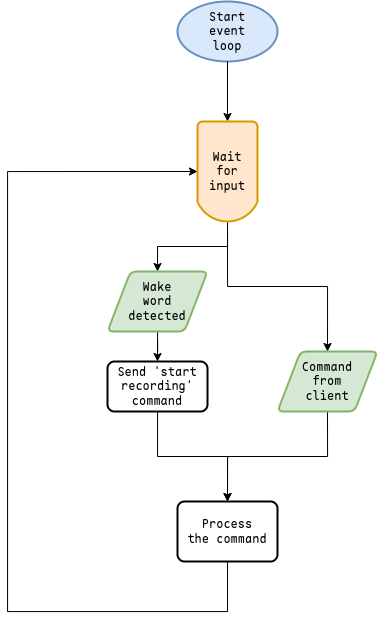
\includegraphics[width=0.5\textwidth]{assets/audio-new}
    \caption{New audio system}
    \label{chart:audio-new}
  \end{figure}
\end{figure}

With the new system, the recording happens on the backend, as does the wake word detection ---
to achieve this, a recording microservice was created, using the following trait:

\begin{minted}{rust}
pub trait RecordingService {
    async fn start(&self) -> Result<()>;
    async fn stop(&self) -> Result<Bytes>;
}
\end{minted}

\subsection{Protocol Updates}
With the new audio recording redesign, rapid full-duplex communication was required, making HTTP no longer a viable option.
While it is technically possible to achieve full-duplex communication using techniques such as Server-Sent Events or WebSockets over HTTP,
switching to raw TCP proved to be much simpler and more effective.
Raw TCP communication allows both the server and client to send messages simultaneously ---
for example, the server could send a response while the client is sending a request to start a new recording.

\subsection{Local Recorder Implementation}
CPAL\footnote{Cross-Platform Audio Library \cite{cpal}} is a Rust library that provides easy access to the audio interface of the system,
allowing one to record audio from Rust code. Using Hound\footnote{Hound \cite{hound}}, the output of CPAL could be encoded into a WAV file
to be sent to the transcription microservice. However, integrating CPAL's inherently synchronous and non-thread safe \texttt{Stream} into an asynchronous API
proved to be challenging, as Rust does not allow synchronous code to run inside asynchronous context, due to concerns for memory safety and avoiding data racing.

\subsection{Temporary Unsafe Implementation}
CPAL's \texttt{Stream} is not thread-safe because it does not implement the \texttt{Send} and \texttt{Sync} traits.
A very intuitive but improper way to circumvent the constraints is to simply implement an unsafe wrapped for \texttt{Send} and \texttt{Sync};
this was done as an interim stopgap measure to allow work to be done on other parts of the project while deliberating about how to implement a proper asynchronous wrapper.
This inherently violates the compiler's thread-safety guarantees, but is acceptable as long as there is only one instance of the local recorder (so only one client).

\begin{minted}{rust}
pub struct UnsafeSendSync<T>(pub T);
unsafe impl<T> Sync for UnsafeSendSync<T> {}
unsafe impl<T> Send for UnsafeSendSync<T> {}
\end{minted}

\subsection{Isolation of Synchronous Recording}
The day after implementing the \texttt{UnsafeSendSync} wrapper for CPAL's \texttt{Stream}, it was decided to simply isolate the \texttt{Stream}
into its own dedicated synchronous thread, separate from the async interface, and communicate using a shared buffer, which could safely be sent across threads./
This buffer was a 10-minute long ring buffer, which means that after 10 minutes of recording, it would overwrite the first samples of the recording.
10 minutes was chosen as the cut-off because it seems unrealistic that someone would talk for more than 10 minutes straight to a voice assistant.
Access to this buffer is synchronized using a mutex, and an atomic counter that keeps track of the total number of samples that have been recorder thus far.
Errors that are thrown inside the synchronous thread are sent to the asynchronous interface via a Tokio multi-producer single-consumer channel and propagated upstream.

\subsection{Wake Word Detection}
A wake word, typically the name of the voice assistant (for example, “Hey Siri” or “Okay Google”),
allows hands‑free activation—making the assistant significantly more convenient to use.
This project utilizes the Porcupine\footnote{Porcupine \cite{porcupine}} library for wake word detection,
and "Ferris" as the wake word, which is the name of the voice assistant, as mentioned in \ref{sec:naming}.
The detection process is implemented in the following code:

\begin{minted}{rust}
fn process_audio_data(
    data: &[f32],
    frame_buffer: &mut Vec<i16>,
    porcupine: &Porcupine,
    wake_word_enabled: &Arc<AtomicBool>,
    is_recording: &Arc<AtomicBool>,
) {
\end{minted}

This function accepts raw audio data and maintains a frame buffer.
Two atomic booleans --- which are thread-safe wrappers for booleans ---
namely \texttt{wake\_word\_enabled} and \texttt{is\_recrding} are passed to this function.

\begin{minted}{rust}
for &sample in data {
    let sample_i16 = (sample * 32767.0) as i16;
    frame_buffer.push(sample_i16);
}
\end{minted}

Audio is stored in floating point samples, which are an easy format
to use for WAV files. These samples need to be converted to 16-bit integers,
because Porcupine expects 16-bit, pulse code modulated signals.
Each converted sample is added to the frame buffer for processing.

\begin{minted}{rust}
if frame_buffer.len() >= porcupine.frame_length() as usize {
    if let Ok(keyword_index) = porcupine.process(frame_buffer) {
\end{minted}

When the buffer has reached a sufficient size, it is processed by Porcupine;
the process method returns a keyword index which can then be used to determine what the outcome was.

\begin{minted}{rust}
if keyword_index >= 0 && wake_word_enabled.load(Ordering::Relaxed) {
    is_recording.store(true, Ordering::Relaxed);
}
frame_buffer.clear();
\end{minted}

A non-negative keyword index means that a wake word was successfully detected.
If wake word detection is enabled, the system transitions to recording mode.
The frame buffer is cleared afterward to prepare for the next batch.
This cycle continues, allowing continuous monitoring for wake word occurrences.
\newline
\begin{figure}[H]
    Below is a flowchart overview showcasing the overall audio recording system, including wake word detection:

    \begin{figure}[H]
        \centering
        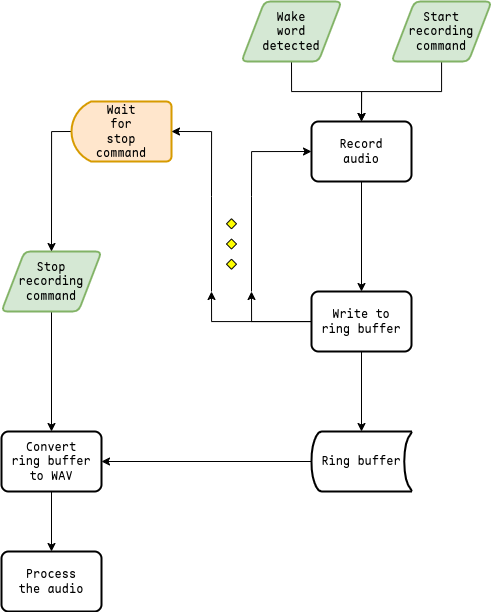
\includegraphics[width=0.5\textwidth]{assets/wakeword.png}
        \caption{Audio recording system and wake word detection}
    \end{figure}
    
    Recording starts when the wake word is detected or the \texttt{start recording} command is received.
    Any recorded audio data is written into a ring buffer, while the \texttt{stop recording} command is awaited in parallel.  
    When the recording is stopped, the captured audio data is extracted from the ring buffer,
    converted into WAV format, and sent to be transcribed by speech-to-text.
\end{figure}

\section{Protocol Updates}
Raw TCP made it difficult to separate text from binary data, often requiring extra logic or a custom protocol.
To simplify things, the setup was changed to use WebSockets over TCP.
WebSockets include built-in message types, which makes it easier for both sides to tell whether data is text, binary, or a control message.

\section{Speech-to-Text Transcription}

\subsection{Audio Preprocessing}
Raw audio is often filled with noise and inconsistent volume levels.
Preprocessing techniques --- like spectral subtraction --- can help isolate vocal frequencies and reduce background noise.
Volume is then normalized to a consistent value.
The cleaned up audio is then transformed into numerical features\footnote{Feature in machine learning \cite{feature}}
using methods such as the Mel Frequency Cepstrum\footnote{Mel Frequency Cepstral \cite{mfc}} or spectrograms.

\subsection{Neural Network Analysis}
The preprocessed features are then input into neural networks trained on thousands of hours of voice data,
which map acoustic signals to text.
There are two main types of neural networks used for audio processing,
those being recurrent neural networks\footnote{Recurrent Neural Network \cite{rnn}},
particularly long short-term memory\footnote{Long short-term memory \cite{lstm}} variants,
which process audio sequentially, retaining context over time,
as well as transformers, using self-attention\footnote{Self-attention \cite{self-attention}},
which in turn model relationships across the entire sequence in parallel.
Hybrid models can combine convolutional layers for phoneme recognition with transformers for better and broader interpretation.

\subsection{Decoding Ambiguity}
Neural network outputs are inherently non-deterministic, which introduces some amount of ambiguity in the transcribed text.
Decoding algorithms help resolve some uncertainty, integrating statistical language models
that leverage context to select the most likely transcription.
When dealing with variable-length inputs and timing discrepancies,
connectionist temporal classification\footnote{Connectionist Temporal Classification \cite{ctc}}
is applied to collapse repeated predictions and blank sections, which provides a preliminary aligned sequence.
This output is then further refined by attention-based models,
which focus on ambiguous segments to provide a more accurate and coherent end result.

\subsection{Rust Trait}
The transcription service is defined via a Rust trait:

\begin{minted}{rust}
pub trait TranscriptionService: Send + Sync {
    async fn transcribe(&self, audio: &Bytes) -> Result<String>;
}
\end{minted}

\subsection{OpenAI Whisper}
OpenAI Whisper is an open-source implementation of automatic speech recognition.
The following is a description by OpenAI\footnote{OpenAI Whisper \cite{whisper}}.

"""Whisper is an automatic speech recognition (ASR) system trained on 680,000 hours
of multilingual and multitask supervised data collected from the web.
We show that the use of such a large and diverse dataset leads to improved robustness to accents,
background noise and technical language.
Moreover, it enables transcription in multiple languages,
as well as translation from those languages into English.
We are open-sourcing models and inference code to serve as a foundation for building useful applications
and for further research on robust speech processing."""

Integration in Rust uses the whisper-rs library:

\begin{minted}{rust}
pub struct LocalWhisperClient {
    context: Arc<WhisperContext>,
}

impl LocalWhisperClient {
    pub fn new(model: impl Into<String>, use_gpu: bool) -> Result<Self> {
        let mut params = WhisperContextParameters::default();
        params.use_gpu = use_gpu;
        let context = Arc::new(
            WhisperContext::new_with_params(&model.into(), params)?
        );
        Ok(Self { context })
    }
}
\end{minted}

This code instantiates a new \texttt{LocalWhisperClient}, using all default parameters besides enabling GPU processing
if the user has configured it to be enabled.
The GPU is much faster than the CPU when running machine learning models, hence why it can be used.

\section{Parsing}
Parsing is the process of analyzing text input and converting it
into a structured format representing its meaning, or the intent that the user most likely had ---
in order to determine which actions should be performed.
This can be accomplished using natural language processing,
be that a simple rule-based parser or a more advanced natural language understanding (NLU) machine learning system.
Rule-based parsing involves matching specific patterns in the input ---
using techniques such as regular expressions or Rust's \texttt{match} statement --- to extract structured data.
In contrast, NLU-based parsing leverages machine learning models, which can be described to actually "understand"
the underlying natural language, hence being able to provide much better results when it comes to intent parsing.

\subsection{Action}
An \texttt{Action} encapsulates the parsed result, including intent, entities, and the original input text:

\begin{minted}{rust}
pub struct Action {
    pub intent: Intent,
    pub entities: Vec<Entity>,
    pub text: String,
}
\end{minted}

An IntentKind is the actual intent that the parser thinks the user wants to perform, while the confidence
is the probability of this intent being correct. Since a rule-based parser is a deterministic pattern matching function,
it does not have a confidence score, hence why \texttt{confidence} is wrapped in an \texttt{Option}.

\begin{minted}{rust}
pub struct Intent {
    pub name: IntentKind,
    pub confidence: Option<f32>,
}

pub enum IntentKind {
    LlmQuery,
    SetTimer,
    WeatherQuery,
    DecreaseVolume,
    IncreaseVolume,
    SetVolume,
    CloseWindow,
    MaximizeWindow,
    MinimizeWindow,
    SwitchWorkspace,
    ShowDesktop,
    Other(String),
}
\end{minted}

\subsection{Pattern Matching}
A rule-based parser was implemented using Rust's \texttt{match} statement.
It operates very similar to the previosly shown Kotlin \texttt{when} statement, detecting words and patterns in the input.
Below is a simplified demonstration of this \texttt{match} statement.

\begin{minted}{rust}
match input_lower.as_str() {
    x if x.contains("close") => CloseWindow

    x if x.contains("minimize") => MinimizeWindow

    x if x.contains("maximize") => MaximizeWindow

    x if x.contains("timer") || x.contains("alarm") => SetTimer

    x if x.contains("switch") && (x.contains("workspace")
    || x.contains("desktop")) => SwitchWorkspace

    x if x.contains("volume") && x.contains("increase") => IncreaseVolume

    x if x.contains("volume") && x.contains("decrease") => DecreaseVolume

    x if x.contains("volume") && (x.contains("set")
    || x.contains("adjust")) => SetVolume

    x if x.contains("weather") || x.contains("whether")
    || x.contains("heather") => WeatherQuery
    _ => LlmQuery
}
\end{minted}

\subsection{NLU-Based Parser}
An NLU-based solution was implemented using Rasa\footnote{Rasa \cite{rasa}} for more adaptable parsing.
Rasa offers dialogue handling, however, for this project, only the NLU component is used,
and dialogue handling may be considered in the future.
Text inputs are tokenized and undergo feature extraction before being processed by the DIETClassifier,
a transformer model that performs both intent classification and entity extraction.

Entities are extracted using the BIO tagging scheme\footnote{Inside-outside-beginning tagging \cite{bio}},
enhanced with spaCy's \texttt{SpacyEntityExtractor}.
spaCy models perform named entity recognition using statistical techniques trained on corpora such as OntoNotes.
The final output includes the identified intent with a confidence score and a list of labeled entities.
This output is then transformed into an \texttt{Action} object for downstream use.

\section{Geocoding}
The geocoding service translates text-based location names into geographic coordinates.
It creates \texttt{GeocodeResponse} objects, which can later be used for weather queries.
Each request requires latitude, longitude, and an API key, with optional parameters for \texttt{units}, \texttt{exclude}, and \texttt{lang}.
An implementation of the geocoding service was a Nominatim\footnote{Nominatim \cite{nominatim}} client;
Nominatim is the internal search engine used by OpenStreetMap to convert addresses into coordinates,
and they provide a public API for it, which is available for free and works quite well, so there was no need for another implementation.

\section{Weather}
Querying the weather is a typical feature of voice assistants, so it was implemented here as well;
the people at OpenWeatherMap are generous enough to provide 1,000 free calls to their weather API every day,
so there was no need to set up a payment system or create another implementation of the weather service.
The weather service is one of the simplest in the project --- it queries the OpenWeatherMap API
and deserializes the response into Rust structs using the serde library.

\section{Timers}
Timers are among the first features associated with a voice assistant, making proper implementation essential.
Timer functionality is achieved by spawning a new Tokio task that waits for the specified duration;
upon expiration, a desktop notification is sent to indicate that the timer has finished.

\begin{minted}{rust}
pub trait TimerService: Send + Sync {
    async fn set(&self, duration: Duration, description: String) -> Result<String>;
}
\end{minted}
Each timer requires a \texttt{Duration} and a description,
which specifies the output message when the timer completed.

\section{Raspberry Pi Setup}
The voice assistant was designed to be deployed on a Raspberry Pi,
whether it's a dedicated node in a smart home or just a helpful assistant on someone's desk.
Given the Raspberry Pi's very limited hardware resources,
particular care had to be taken to reduce its local computational load.
Where possible, services were designed with remote execution in mind,
to allow them to run on low-end hardware.
Alpine Linux\footnote{Alpine Linux \cite{alpine}}
was chosen as the operating system for its minimalism, fast boot times, and low memory usage.

\subsection{Installation Procedure}
To install the system, an aarch64 Raspberry Pi image was downloaded from the Alpine Linux website
and then flashed onto a microSD card using \texttt{dd}:
\begin{minted}{bash}
sudo dd if=alpine-rpi-*.img of=/dev/sdX bs=4M status=progress
\end{minted}

The built-in \texttt{setup-alpine} script was executed to configure basic settings on the system.
The script guided configuration of essential system settings including:
keyboard layout, hostname, timezone, network configuration, and partitioning.

KDE Plasma was then installed to provide a full desktop environment:
\begin{minted}{bash}
apk add plasma-desktop sddm xdg-utils
rc-update add sddm
\end{minted}
This choice was deliberate, since the reference frontend is written in Qt,
which is well integrated into KDE Plasma.

Connecting the RGB LED and physical buttons was done using the RPPAL\footnote{Raspberry Pi Peripheral Access Library \cite{rppal}} Rust library ---
if a recording was active the LED would light up green and if an error occured it would light up red.
This could be configured further, but is not neccessary because errors are reported via text or audio either way.